\begin{figure}[t!]
    \centering
    \captionsetup{type=figure}
    \begin{subfigure}[t]{0.48\linewidth}
        \centering
        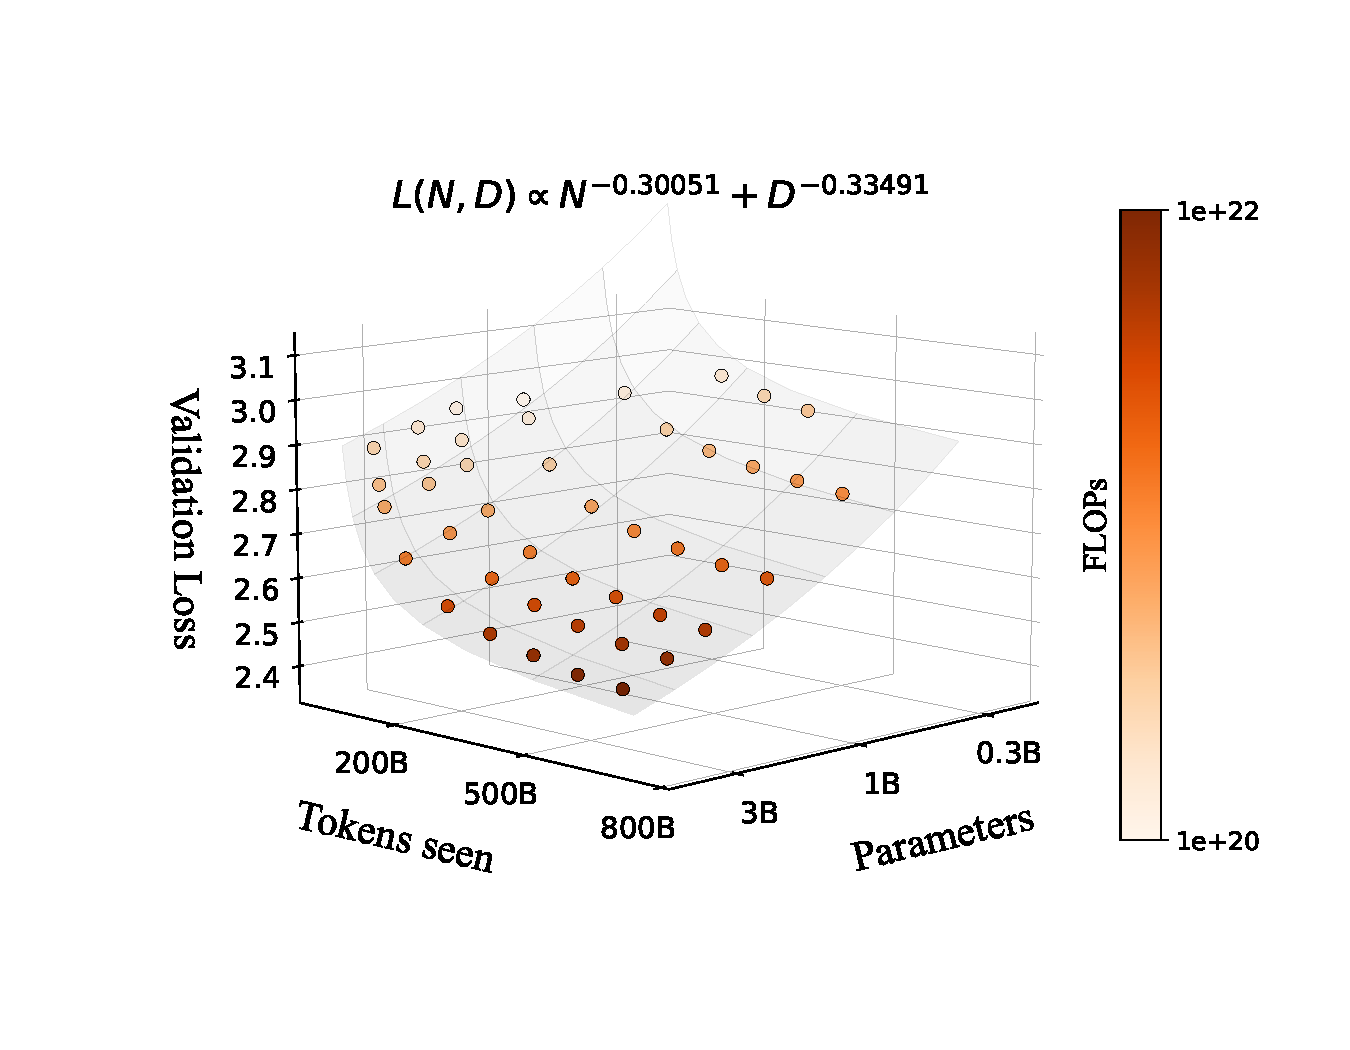
\includegraphics[width=1.02\linewidth]{assets/early/3d_scaling_early.pdf}
    \end{subfigure}
    \hfil
    \begin{subfigure}[t]{0.48\linewidth}
        \centering
        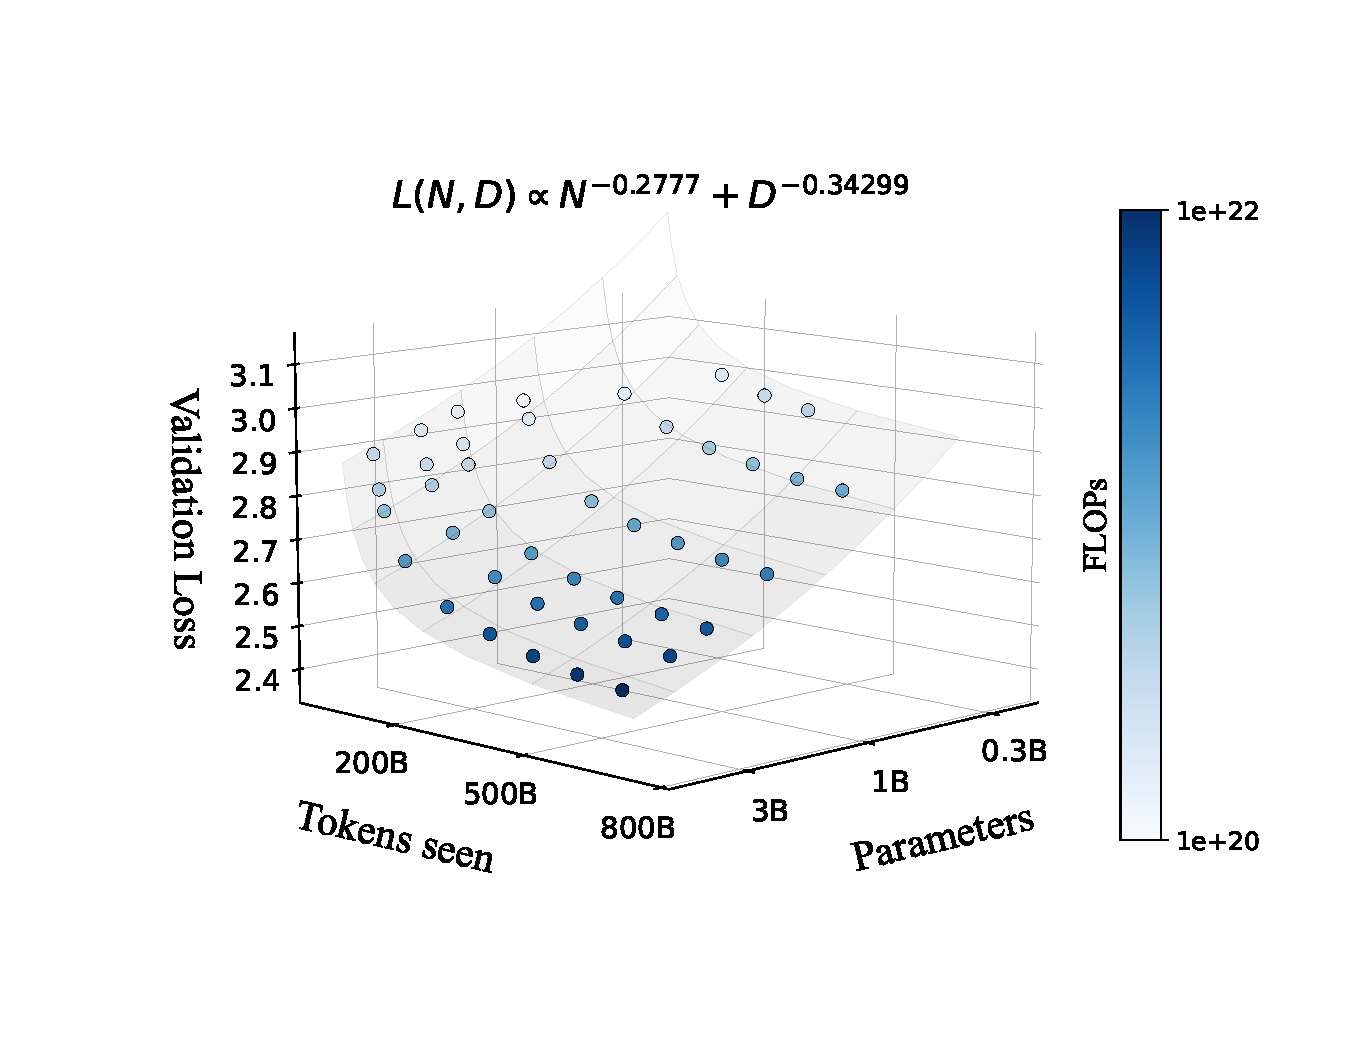
\includegraphics[width=1.02\linewidth]{assets/early/3d_scaling_late.pdf}
    \end{subfigure}
    \vspace{5pt}
    \setlength{\fboxsep}{0.5pt}
    \setlength{\fboxrule}{0pt}
    \caption{\textbf{早期融合和 \fbox{\colorbox{CustomC_Light1!20}{\strut
    早期融合}} 和 \fbox{\colorbox{CustomD_Light1!20}{晚期融合\strut}}
    本地多模态模型的规模规律。} 每个点代表一个模型(300M 到 3B
    参数),在不同的 \edit{标记数量}(250M 到 400B)上训练。我们
    报告在 \edit{交替(Obelics)、图像-标题(HQITP)和仅文本数据
    (DCLM)} 上的平均交叉熵损失。}
    \label{fig:early_vs_late_scaleflops_3d}
\end{figure}
